\section{Preliminary Results}

In this section, we will discuss some of our preliminary results. 
We first randomly split all 7841 labeled images into two parts: 
training set (4953 images) and validation set (2538 images). 
For now, we have conducted three experiments on object detection, including using a pre-trained yolo model, using a fine-tuned tiny yolo model based on our training set and using a pre-trained Faster-RCNN model. All the experiments are conducted on AWS using a g2.2xlarge instance with GRID K520 GPU. We directly use the Yolo implementation from Darknet \footnote{\url{https://github.com/pjreddie/darknet.git}} and the Faster R-CNN python implementation \footnote{\url{https://github.com/rbgirshick/py-faster-rcnn}}.

In terms of evaluating the object detection results, KITTI benchmark requires a minimum overlap of 70\% for cars and 50\% for pedestrians. It also has three kinds of difficulties: easy, moderate and hard. Difficulties are defined as follows:

\begin{table}[h!]
\centering
\begin{tabular}{ c | c | c | c }
\hline
Difficulty & Min. bounding box height & Max. occlusion level & Max. truncation \\
\hline \hline
Easy & 40 Px & Fully visible & 15\% \\
Moderate & 25 Px & Partly occluded & 30\% \\
Hard & 25 Px & Difficult to see & 50\% \\
\hline
\end{tabular}
\caption{Different Difficulties Requirements}
\end{table}

The pre-trained yolo model is trained on Pascal VOC 2012 and 2007 dataset \footnote{\url{http://pjreddie.com/darknet/yolo/}}. It supports about 20 object categories including car and people (corresponding to pedestrian). However it don't support cyclist category. So in all the following experiments, we only evaluate the performance for cars and pedestrians.

For now, we only detect cars and pedestrians in images. Considering the limitation of time and compute power, we choose the tiny yolo model to fast tune. Tiny yolo model is very similar to yolo model, but only contains 8 convolutional layers. We use convolutional weights that are pre-trained on ImageNet classification task as initial weights. Fine tuning tiny yolo model makes it possible to benefit from the features the model has learnt previously and speed up training. It took about 16 hours to train tiny yolo after 10,000 iterations.


The pre-trained Faster-RCNN model is trained on Pascal VOC 2007 dataset. It is able to detect cars and pedestrians and also lacks of supports for cyclists.

% \begin{figure}[H]
% \begin{subfigure}{.5\textwidth}
%     \centering
%     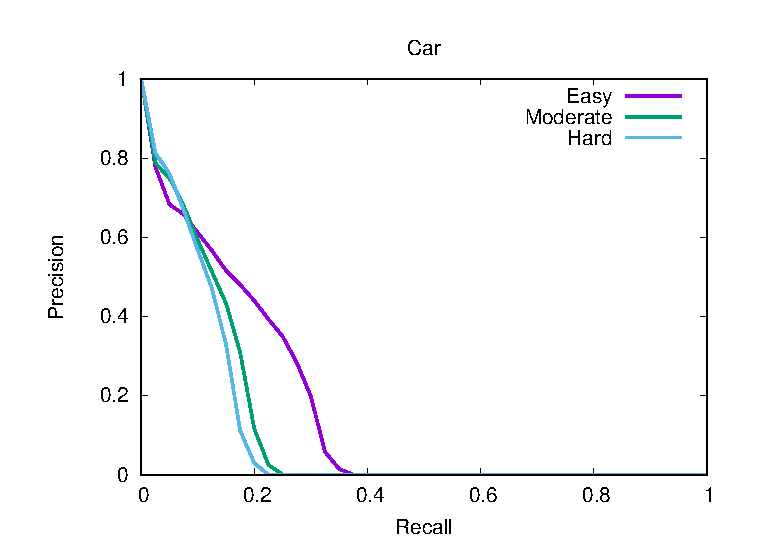
\includegraphics[width=1.0\linewidth]{img/yolo_Nov_4/plot_valid/car_detection.eps}
%     % \caption{Seed = 4}
% \end{subfigure}%
% \begin{subfigure}{.5\textwidth}
%     \centering
%     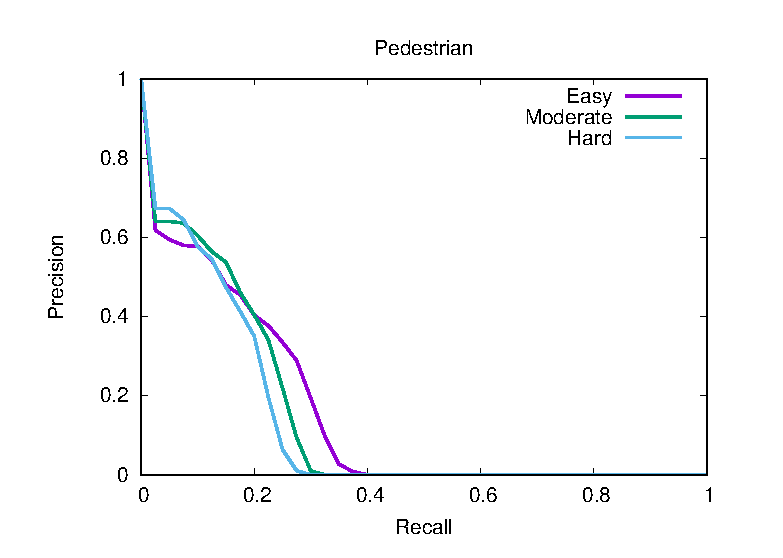
\includegraphics[width=1.0\linewidth]{img/yolo_Nov_4/plot_valid/pedestrian_detection.eps}
%     % \caption{Seed = 4}
% \end{subfigure}
% \caption{Using a Pre-Trained Yolo Model}
% \begin{subfigure}{.5\textwidth}
%     \centering
%     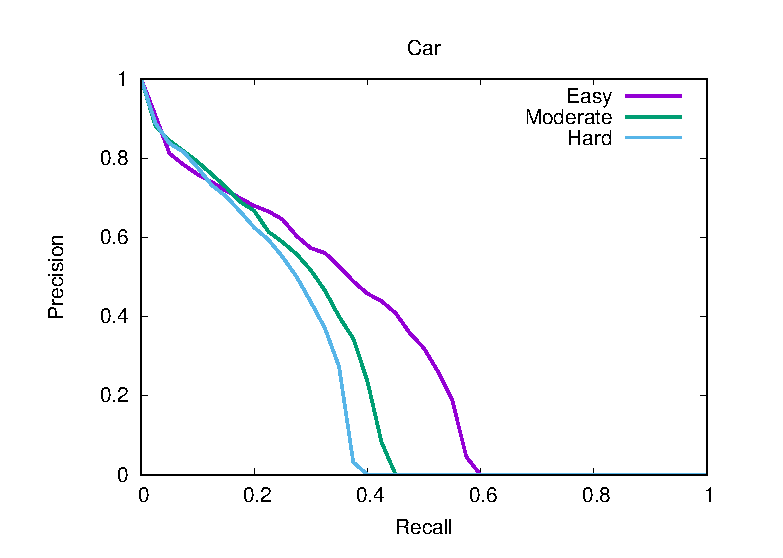
\includegraphics[width=1.0\linewidth]{img/yolo_Nov_9/plot_valid/car_detection.eps}
%     % \caption{Seed = 4}
% \end{subfigure}%
% \begin{subfigure}{.5\textwidth}
%     \centering
%     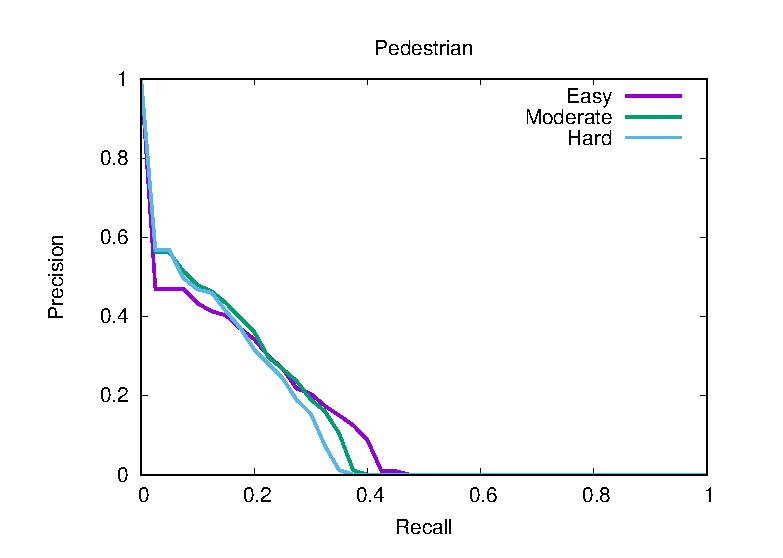
\includegraphics[width=1.0\linewidth]{img/yolo_Nov_9/plot_valid/pedestrian_detection.eps}
%     % \caption{Seed = 4}
% \end{subfigure}
% \caption{Using a Tiny Yolo Model Trained on Our Dataset}
% \begin{subfigure}{.5\textwidth}
%     \centering
%     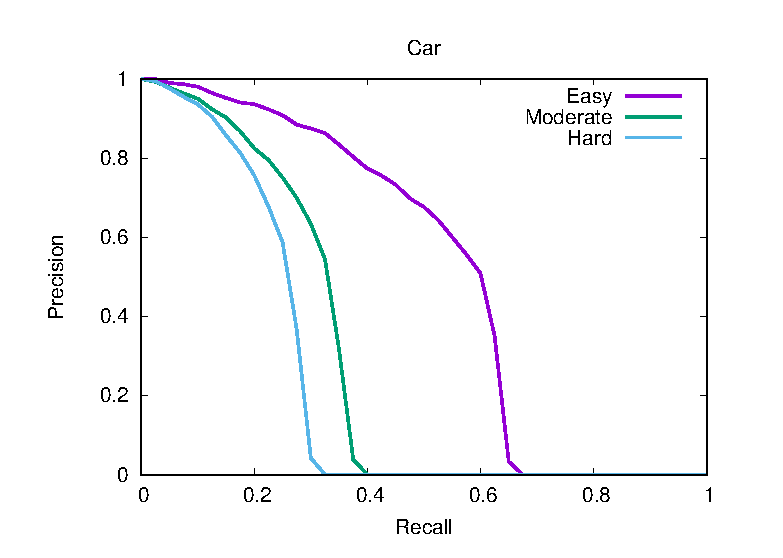
\includegraphics[width=1.0\linewidth]{img/FRCNN_Nov_8/plot_valid/car_detection.eps}
%     % \caption{Seed = 4}
% \end{subfigure}%
% \begin{subfigure}{.5\textwidth}
%     \centering
%     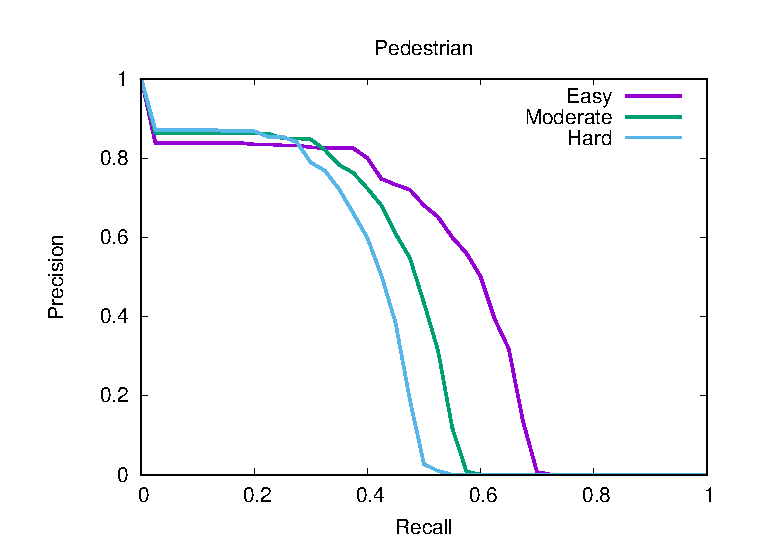
\includegraphics[width=1.0\linewidth]{img/FRCNN_Nov_8/plot_valid/pedestrian_detection.eps}
%     % \caption{Seed = 4}
% \end{subfigure}
% \caption{Using a Pre-Trained Faster-RCNN Model}
% \end{figure}

\begin{figure}[H]
\begin{subfigure}{.34\textwidth}
    \centering
    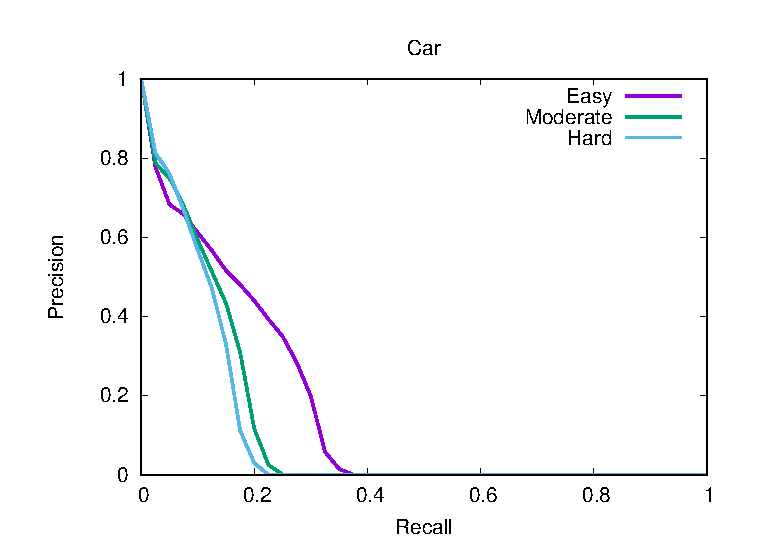
\includegraphics[width=1.0\linewidth]{img/yolo_Nov_4/plot_valid/car_detection.eps}
    \caption{Pre-Trained Yolo Model}
    % \caption{Seed = 4}
\end{subfigure}%
\begin{subfigure}{.34\textwidth}
    \centering
    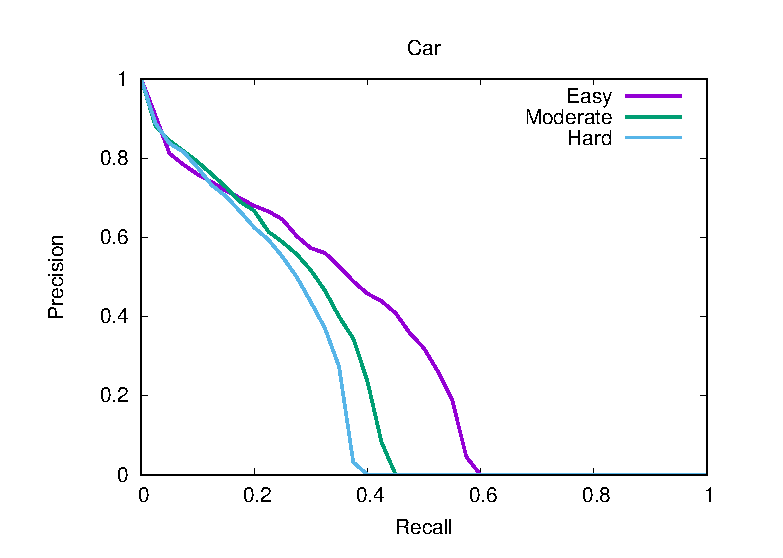
\includegraphics[width=1.0\linewidth]{img/yolo_Nov_9/plot_valid/car_detection.eps}
    % \caption{Seed = 4}
    \caption{Fine-Tuned Tiny Yolo Model}
\end{subfigure}%
\begin{subfigure}{.34\textwidth}
    \centering
    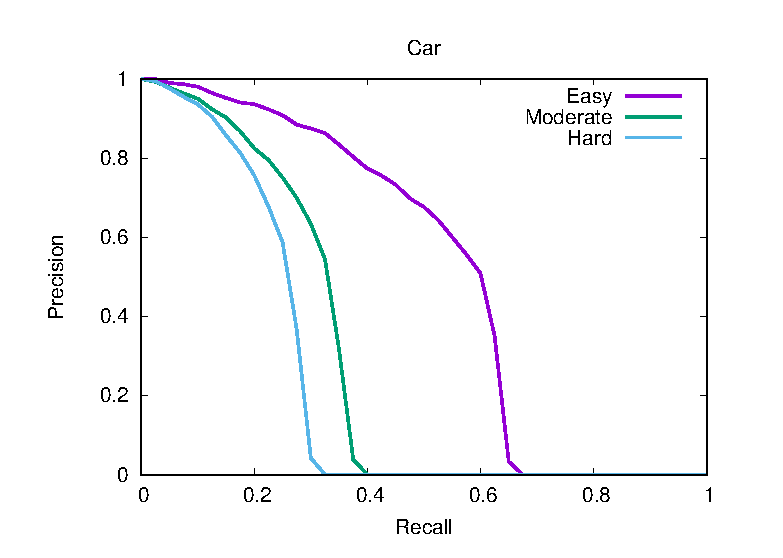
\includegraphics[width=1.0\linewidth]{img/FRCNN_Nov_8/plot_valid/car_detection.eps}
    \caption{Pre-Trained Faster-RCNN Model}
\end{subfigure}
\caption{Car Detection}
\end{figure}

\begin{table}[h!]
\centering
\begin{tabular}{ c | c | c | c }
\hline
Method & Easy & Moderate & Hard \\
\hline \hline
Pre-Trained Yolo & 0.204438 & 0.155358 & 0.145101 \\
Fine-Tuned Tiny Yolo & 0.344293 & 0.291823 & \bfseries 0.257863 \\
Pre-Trained Faster-RCNN & \bfseries 0.522754 & \bfseries 0.309875 & 0.248554 \\
\hline
\end{tabular}
\caption{Average Precision on Car Detection}
\end{table}

\begin{figure}[H]
\begin{subfigure}{.34\textwidth}
    \centering
    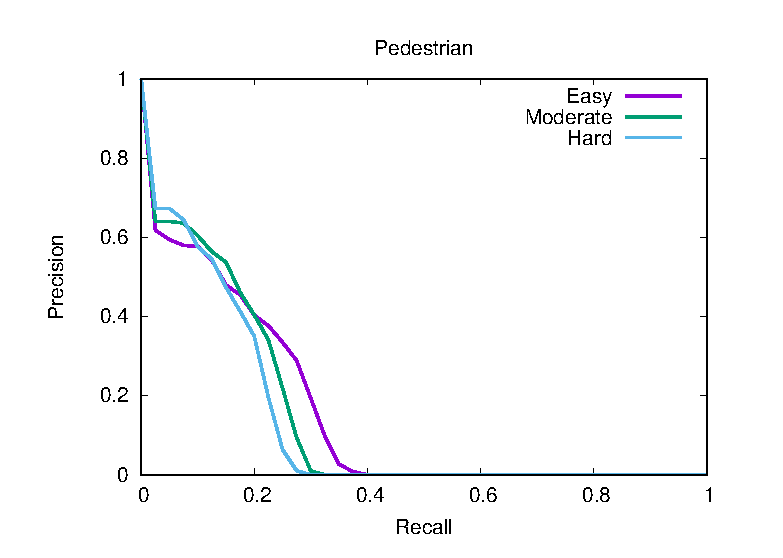
\includegraphics[width=1.0\linewidth]{img/yolo_Nov_4/plot_valid/pedestrian_detection.eps}
    \caption{Pre-Trained Yolo Model}
\end{subfigure}%
\begin{subfigure}{.34\textwidth}
    \centering
    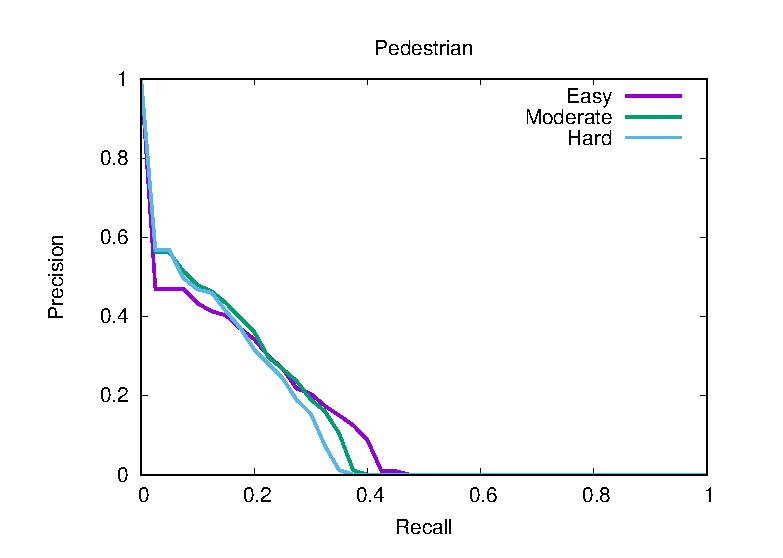
\includegraphics[width=1.0\linewidth]{img/yolo_Nov_9/plot_valid/pedestrian_detection.eps}
    \caption{Fine-Tuned Tiny Yolo Model}
\end{subfigure}%
\begin{subfigure}{.34\textwidth}
    \centering
    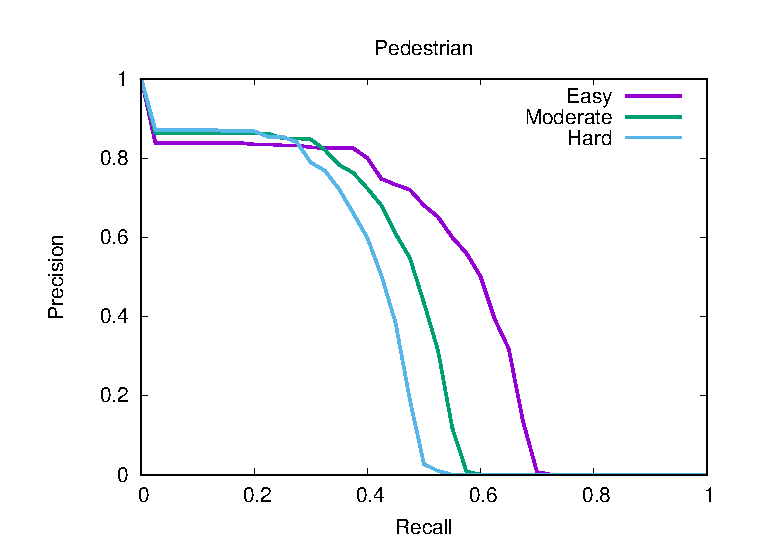
\includegraphics[width=1.0\linewidth]{img/FRCNN_Nov_8/plot_valid/pedestrian_detection.eps}
    \caption{Pre-Trained Faster-RCNN Model}
\end{subfigure}
\caption{Pedestrian Detection}
\end{figure}

\begin{table}[h!]
\centering
\begin{tabular}{ c | c | c | c }
\hline
Method & Easy & Moderate & Hard \\
\hline \hline
Pre-Trained Yolo & 0.197457 & 0.183323 & 0.175022 \\
Fine-Tuned Tiny Yolo & 0.187898 & 0.184558 & 0.176187 \\
Pre-Trained Faster-RCNN & \bfseries 0.498992 & \bfseries 0.429862 & \bfseries 0.377569 \\
\hline
\end{tabular}
\caption{Average Precision on Pedestrian Detection}
\end{table}

As we can see from the precision-recall curve and the average precision results, for pedestrians, Faster-RCNN outperforms yolo models a lot in all three difficulity levels. And a fine-tuned tiny yolo model on our dataset shows no improvement compared with the pre-trained yolo model. For cars, Faster-RCNN outperforms yolo models in easy level. And our fine-tuned tiny yolo model shows great improvement in all three difficulity levels compared with the pre-traiend yolo model. And
in terms of predicting speed, the fine-tuned tiny yolo can achieve about 70 fps and the pre-trained Faster-RCNN can only achieve about 2 fps.
